%!TEX root = ../../secondYearReport.tex


\paragraph{Work package 4 progress}

% \subparagraph{Improved Models from Real-Time Regression with Latent Contact Type Inference (T4.1)}%(TUD 8.5PM, ??PARTNERS)}
% 
% %IIT
% Within T4.1 IIT developed a theoretical framework for estimating whole-body
% dynamics from distributed multimodal sensors \cite{Nori2015}. Considered sensors
% include joint encoders, gyroscopes, accelerometers and force/torque sensors.
% Estimated quantities are position, velocity, acceleration and (internal and
% external) wrenches on all the rigid bodies composing the robot articulated
% chain. The estimation procedure consists of an extended Kalman filter (EKF)
% which gives the a-posteriori estimation given all the available measurements.
% Computational efficiency is obtained by formulating the Kalman filter
% update-step with a sparse Bayesian network. Experiments for validating the
% proposed theoretical framework have been conducted on a leg of the iCub humanoid
% robot. The iCub is an ideal platform for the proposed experiment given its
% distributed force, torque, linear acceleration and angular velocity sensors.
% Results have shown the accuracy and the computational efficiency of the proposed
% method. The theoretical framework has been implemented in an open source
% software (see also Section \ref{sec:T15}).
% 
% %TUD
% %LMProMPs and Model-free ProMPs
% TUD extended their probabilistic movement primitive (ProMP) approach in two
% ways. First, a mixture model approach that learns a shared latent structure of
% related tasks from demonstrations was developed. The shared structure is encoded
% by a multi-modal vector that modulates the probabilistic primitives. Both, the
% probabilistic primitives as well as their activations (i.e., the latent
% variable) are learned from demonstrations. In a table tennis ball prediction
% tasks this latent variable modulated the slope and the waviness of the ball
% trajectory. In a Kuka robot arm reaching task, the approach was used to learn
% bi-modal reaching trajectories that avoid an obstacle placed in front of the
% robot. This work is detailed in Deliverable D4.2 and will be presented at the
% IEEE conference on Robotics and Automation in May in Seattle, USA
% \cite{Rueckert_2015}. 
% 
% In a second extension of ProMPs, TUD developed a model-free control method that
% can be trained from demonstrations and generates time-varying feedback control
% gains that reproduces the demonstrations. In this approach a joint distribution
% over states, sensory feedback (e.g., measured joint torques or contact forces)
% and controls is learned. In conditioning on the current state the next-state
% control-law can be computed in closed form approximating the true forward
% dynamics through local linearizations given the demonstrations. TUD evalated
% this model-free ProMP method on the humanoid robot iCub in lifting objects. A
% conference paper is currently under review. 


\subparagraph{Inferring the Operational Space and Appropriate Controls with Multiple Contacts (T4.2) (..., TUD: 6PM, ...)}%(TUD 4PM, ??PARTNERS)}

%TUD

%Elmar 
During year two, TUD and JSI investigated the effect of supportive contacts on 
postural control. First results were presented during the second year review 
meeting (Task T2.4 on Human contact choice and learning through physical 
interaction). During year three, we collected a large dataset of more than 
$9.000$ reaching movements in $20$ subjects. To analyze the data TUD developed a 
probabilistic model which extends classical statistical tests (ANOVA test of 
contact locations and target locations, movement onsets, etc.). The 
probabilistic model allows for detailed investigations of movement kinematics in 
a spaciotemporal domain and extends classical techniques that rely on scalar 
descriptors of the complex motion patterns. In whole body adaptation 
experiments, shown in Figure \ref{fig:subFigContactLocationsAllSubjects}, TUD 
and JSI found strong correlations between both arms and the trunk. These 
correlations were used to predict the reaching motion from early phase 
observations of the supportive contact motion. The results suggest that postural 
control predicts and precedes goal-directed movements, which has the potential 
to impact pre-tests of central nervous system disorders like dementia, 
Alzheimer's or Parkinson's disease that are less prone to factors like stress, 
sleep deprivation and age compared to the classical cognitive tests. A pre-print 
of a paper that was submitted for review to Scientific Reports is given in 
Deliverable D2.2.

\begin{figure}%[t]
\centering
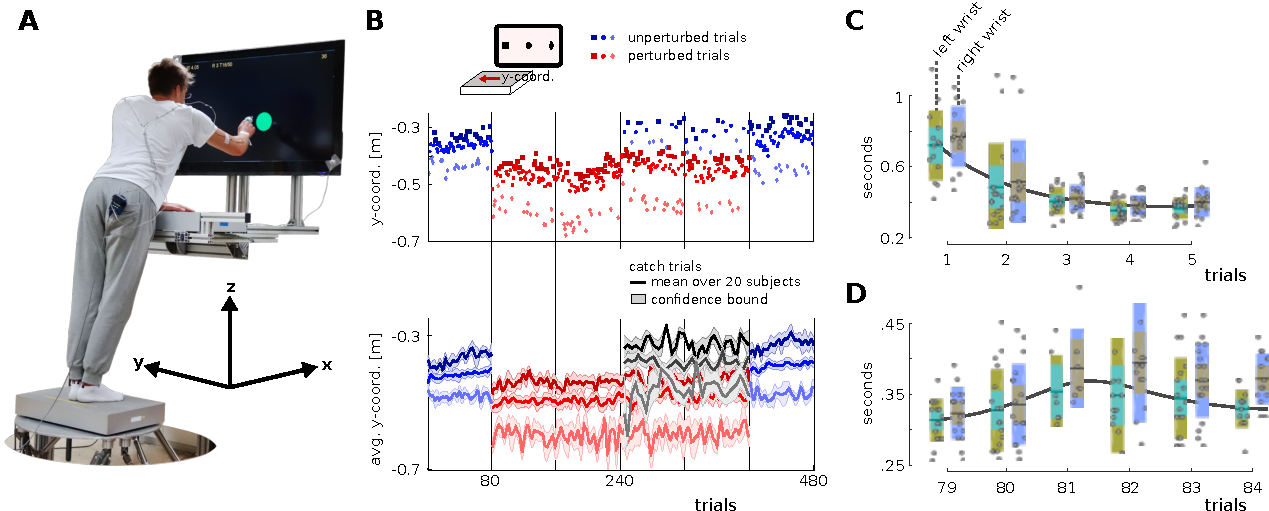
\includegraphics[width=\textwidth]{images/Figure-1(rueckert)}
%\label{fig:subfig2}
 \caption[Human reaching experiment with target dependent contacts and synchronized arm motions.]{\textbf{Experiment, target dependent contacts and synchronized arm motions.} \textbf{A)} Experimental setting. 
 \textbf{B)}  The top row shows contact locations for a single representative subject 
 and the bottom row shows the mean and the confidence bound over all $20$ participants. 
 The first $80$ trials and the last $80$ trials are unperturbed sessions. 
 Catch trials were initiated during trials $240$ to $400$ and are denoted by the black lines in \textbf{B}.
 \textbf{C)} Illustration of the movement onsets of the wrists for the first five trials. 
 \textbf{D)} Movement onsets for the first six trials transitioning to the perturbed session. 
}
\label{fig:subFigContactLocationsAllSubjects}
\end{figure}

In ongoing work, TUD and JSI investigate how such probabilistic models can predict when 
and how to make supportive contacts in robot reaching tasks. Our goal is to 
reproduce the correlated reaching and supportive contact motions in the ICub robot. 
In addition to the target dependent contact locations, a module that predicts 
when to initiate a supportive contact will be developed. This model will make 
use of the estimated center of pressure using the two force/torque sensors in the 
ankles. 

\begin{figure}
\centering
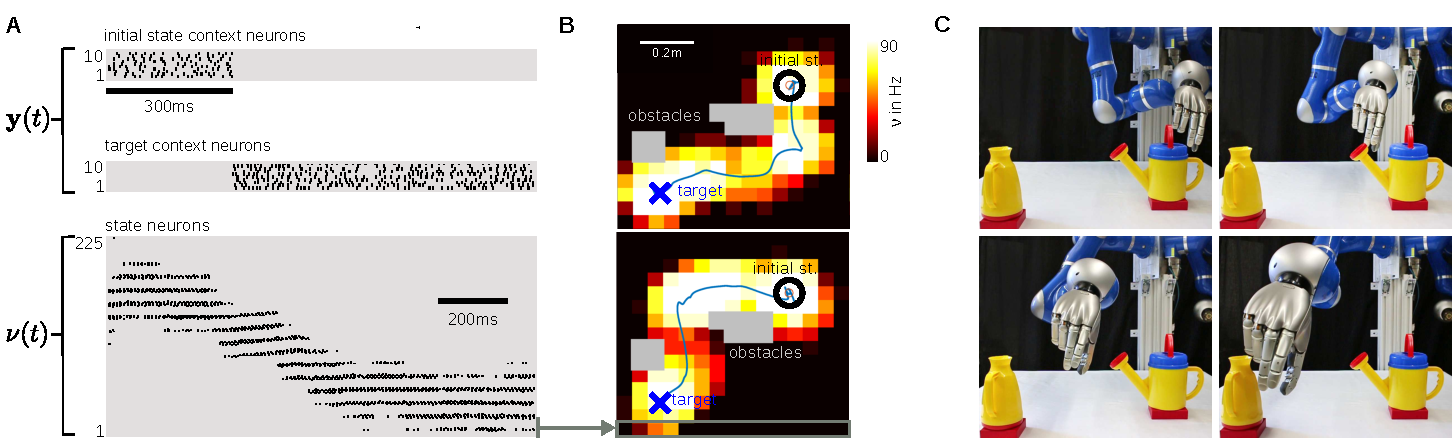
\includegraphics[width=\textwidth]{images/KukaLearnedModelObstacles}
%\label{fig:subfig2}
 \caption[Planning in spkining neural networks with multiple constraints on a Kuka robot.]{\textbf{Planning with multiple constraints on a real robot.} {\bf A)} Generated 
spike train (top: context neurons, bottom: state neurons) after contrastive 
divergence learning of the transition model. {\bf B)} Two sampled movement plans 
solving the obstacle avoidance task. {\bf C)} Snapshots of the executed movement 
on the real robot.
}
\label{fig:exp_kukaRueckert}
\end{figure}

In another approach, TUD investigated computational models of operational space 
control in rodents using spiking neural networks. While this study is more of a 
fundamental type and does not directly provide concrete algorithms for humanoid 
robot control, it has interesting potentials for the challenging tasks in 
CoDyCo. Concretely, in spiking neural networks arbitrary-shaped obstacles can be 
modeled, non-linearities in the transition model due to contacts can be learned 
and movement plans can computed much faster then real-time through exploiting 
local-only dependencies. These advantages were evaluated in target-reaching task 
in a Kuka robot arm. For that TUD developed learning algorithms grounded in the 
theory of probabilistic inference to train the recurrent spiking neural network 
from human demonstrations. The training data was collected in kinesthetic 
teaching. After the training, the network model was used to plan goal-directed 
task space trajectories that avoid obstacles in the three-dimensional space. Two 
example movements and the corresponding neural activity are illustrated in 
Figure \ref{fig:exp_kukaRueckert}. For details on the approach we refer to 
Deliverable D4.1. A manuscript on this work was accepted for publication in 
Scientific Reports~\cite{Rueckert_SR_2016} (impact factor 5.578 in 2014). 

In a student's master thesis, TUD extended the model to jointly model 
configuration and task spaces. This extension is based on factorized population 
codes and allows for applications to high-dimensional robot systems. In ongoing 
work, TUD will test the learning algorithms of the spiking network in the ICub 
robot.    



% \subparagraph{Generalizing and Improving Elementary Tasks with Contacts (T4.3)}%(TUD 6PM, ??PARTNERS)}
% 
% The advent of robots in our every day life can only be accomplished with
% reliable mechanisms for movement generation.  Movement Primitives (MP) are a
% well-established approach for representing modular and re-usable robot movement
% generators that can be composed into complex movements.  An easy-to-learn
% representation of the primitive is, additionally, the key of recent imitation
% and reinforcement learning successes. Current MPs approaches offer viable
% properties such as concise representations of the inherently continuous and
% high dimensional space of robot movements, generalization capabilities to novel
% situations, temporal modulation of the primitive, sequencing of primitives,
% coupling between the degrees of freedom of the robot, and controllers for real
% time execution. However, no single MP framework exists that offers all these
% properties.  During year two, TUD extended previous results on modeling stochastic movements \cite{Paraschos2013,Paraschos2013a}, where a journal version is currently under review. 
% 
% \definecolor{light-gray}{rgb}{0.91,0.9,0.88}
% 
% \newcommand{\hockeyImLabel}[3]{%
% \begin{tikzpicture}
% \node[  anchor=south west,inner sep=0,%
%         draw=gray,%
%         %left color=gray,right color=white%
%         %fill=light-gray%
% ] (image) at (0,0){
% \includegraphics[width=0.29\textwidth]{#1}};
% \begin{scope}[x={(image.south east)},y={(image.north west)}]
%     %\draw[help lines,xstep=.1,ystep=.1] (0,0) grid (1,1);
%     %\foreach \x in {0,1,...,9} { \node [anchor=north] at (\x/10,0) {0.\x}; }
%     %\foreach \y in {0,1,...,9} { \node [anchor=east] at (0,\y/10) {0.\y}; }
%     \node [fill=white,opacity=0.6,above right,font=\large] at (0.01,0.01) {#2};
%     \node [fill=white,opacity=0.6,below left,font=\large] at (0.99,0.99) {#3};
% \end{scope}
% \begin{scope}[x={(image.south east)},%
%               y={(image.north west)},% 
%               on background layer]
%     %\path[fill=light-gray] (0,0) rectangle (1,1);
%     \path[outer color=light-gray,inner color=white] (0,0) rectangle (1,1);
%     \draw[gray,opacity=0.15,xstep=.1,ystep=.1] (0,0) grid (1,1);
% \end{scope}
% \end{tikzpicture}%
% }
% 
% \begin{figure*}
% \centering
% \hockeyImLabel{./sections/WP4/pics_alex/Setup_tr_sm.png}{$a$}{Setup}
% \hockeyImLabel{./sections/WP4/pics_alex/Distances_tr_sm}{$b$}{Distance}
% \hockeyImLabel{./sections/WP4/pics_alex/HockeyAngle_tr_sm}{$c$}{Angle}
% 
% \vspace{0.2em}
% 
% \hockeyImLabel{./sections/WP4/pics_alex/Joint_tr_sm}{$d$}{Union}
% \hockeyImLabel{./sections/WP4/pics_alex/Combined_tr_sm}{$e$}{Combination}
% \hockeyImLabel{./sections/WP4/pics_alex/Joint-LeftRight_tr_sm.png}{$f$}{Conditioning}
% 
% \caption{Robot Hockey. The robot shoots a hockey puck. We demonstrate ten straight
% shots for varying distances and ten shots for varying angles. The
% pictures show samples from the ProMP model for straight shots ($b$)
% and angled shots ($c$). Learning from the union of the two data sets yields a model
% that represents variance in both, distance and angle ($d$). Multiplying
% the individual models leads to the combined a model that only reproduces shots
% where both models had probability mass, in the center at medium distance
% ($e$). The last picture shows the effect of conditioning on only left
% and right angles ($f$).}
% \label{fig:Robot-Hockey}
% 
% \end{figure*}
% 
% TUD incorporated all the desirable properties 
% current approaches offer into a single framework and, additionally, TUD 
% introduced new operations on the primitives, such as continuous blending and
% co-activation of multiple primitives.  Most importantly, in this approach, the
% novel co-activation operator is capable of solving multiple tasks concurrently \ref{fig:Robot-Hockey}.
% Furthermore, TUD's approach is capable of reproducing exactly the demonstrated
% variability of the movement and the coupling between the degrees of freedom of
% the robot.  In this approach, called Probabilistic Movement Primitives (ProMPs) \cite{Paraschos2013,Paraschos2013a},
% TUD derived all operations in closed form. In order to use the ProMPs for online
% feedback control, TUD also derived a stochastic feedback controller that
% reproduces exactly the encoded primitive. TUD evaluated and compared this approach
% on several simulated and real robot scenarios.
% 
% Probabilistic movement primitives are a promising approach for learning,
% modulating, and re-using movements in a modular control architecture.  To
% effectively take advantage of such a control architecture, ProMPs support
% simultaneous activation, match the quality of the encoded behavior from the
% demonstrations, are able to adapt to different desired target positions, and
% efficiently learn by imitation. ProMPs meets all of the aforementioned
% requirements.  The desired trajectory distribution of the
% primitive is parametrized by a hierarchical Bayesian model with Gaussian distributions. The
% trajectory distribution can be obtained from demonstrations and 
% simultaneously defines a feedback controller which is used for movement
% execution. Currently, TUD is investigating extensions of the ProMPs framework 
% to tasks that involve 
% contacts with the environment (see T4.1). In addition, TUD started to investigate the improvement of elementary skills encoded in ProMPs with 
% reinforcement learning, where a conference paper was submitted for review.


\subparagraph{Learning the Prioritization of Tasks (T4.4) (..., TUD: 6PM, ...)}%(TUD 3.2PM, INRIA 2PM)}

During the third year, TUD continued its research on learning controllers for 
physical interaction. We presented a novel approach at an international robotics 
conference~\cite{paraschos2015model}. The approach learns and generates 
movements for physical interaction that are trained with imitation learning from 
a small set of demonstrated trajectories. Learning such a model is a non-trivial 
task and therefore we introduced the \textit{model-free} Probabilistic Movement 
Primitives (ProMPs). Here, we learn jointly the movement and the necessary 
actions from a few demonstrations. We derived a variable stiffness controller 
analytically and we extended the ProMPs to include force and torque signals, 
necessary for physical interaction in the CoDyCo scenarios. 

Based on these results we also focused on developing a novel approach for task 
prioritization during year three. Our approach follows the concept of ``soft'' 
priorities, where a task which is lower in the task-hierarchy can controllably 
interfere with a higher-priority task. This concept is applicable to a wide-set 
of problems including balancing and reaching in humanoids with physical contacts 
with the environment. In our approach we dynamically change the priority of each 
task in time and, thus, adapt the behavior of the robot dynamically.  The 
approach utilizes imitation learning to obtain the variance of each task 
movement which is then used as the relative priority of the task. An important 
contribution of our approach shows how we can utilize probabilistic methods to 
analytically derive the tasks priorities from the imitation learning. We relate 
our approach to other state-of-the-art movement prioritization 
approaches~\cite{Peters_AR_2008, lober2015variance} and we show how these 
approaches can be derived under our framework. We provide an alternative point 
of view on movement prioritization that is derived from first-order principles. 
We demonstrated that our approach achieves improved performance and that is 
numerically stable, avoiding singularities. A paper on this approach was 
submitted to a robotics conference.

% During year two, UB continued their research on computed torque control leveraging low-gain control. 
% In computed torque control, robot dynamics are predicted by dynamic models.
% This enables more compliant control, as the gains of the feedback term can be
% lowered, because the task of compensating for robot dynamics is delegated from
% the feedback to the feedforward term.  We already showed that Gaussian process
% regression is an effective method for learning computed torque control, by
% setting the feedforward torques to the mean of the Gaussian process.  During
% the second year of the project, we extended this work by also exploiting the
% variance predicted by the Gaussian process, by lowering the gains if the
% variance is low \cite{Albertoetal14}.  This enables an automatic adaptation of
% the gains to the uncertainty in the computed torque model, and leads to more
% compliant low-gain control as the robot learns more accurate models over time.
% On a simulated 7-DOF robot manipulator, we demonstrated how accurate tracking
% can be achieved, despite the gains being lowered over time, which is illustrated in Figure \ref{fig:meanvariance}.
% 
% \begin{figure}
%   \centering
%   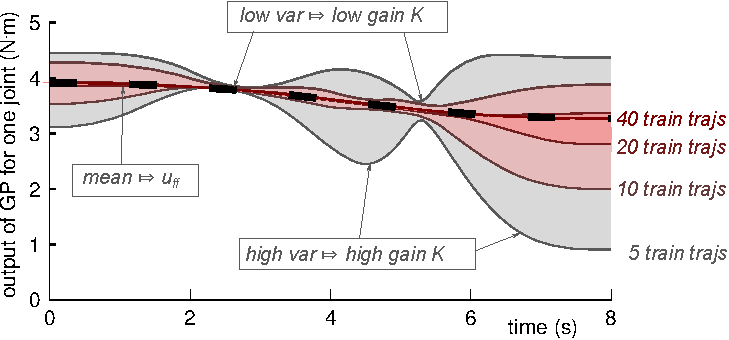
\includegraphics[scale=0.8]{images/meanvariance.pdf}
%   \caption{Mean and variance of the Gaussian process ($\mu \mp 2\sigma$) on
%     the same test trajectory of 8 seconds, after having been trained with 5,
%     10, 20 and 40 training trajectories. With an increasing number of training
%     data, the mean of the GP approaches the true function (black dashed
%     line). The known values for uff are plotted as a black dotted line.}
%   \label{fig:meanvariance}
% \end{figure}
% 
% %!TEX root = ../../secondYearReport.tex

% 1.68 man.months for UPMC on T4.4 

Within T4.4, UPMC studied how to deal with interferences between tasks using machine learning tools. Whole-Body Control methods offer the potential to execute several simultaneous tasks on highly redundant robots, such as humanoids. Unfortunately, task combinations often result in interferences or incompatibilities which generate undesirable behaviors. Prioritization schemes between tasks, such as strict and soft hierarchies, are typically used to manage these interferences but generally require a deal of time consuming and arbitrary tuning.

To circumvent theses issues, UPMC presented a novel framework for defining and optimizing multiple tasks in order to resolve potential interferences prior to task execution. In a first study \cite{lober-HUMANOIDS2014} the tasks are parameterized with Dynamical Movement Primitives, whose parameters are optimized based on a general compatibility principle, which is independent of the robot’s topology, tasks or environment. Two test cases on a simulation of a humanoid robot are used to demonstrate the successful optimization of initially interfering tasks. A video summarizing the outcome of this work can be viewed \href{here}{http://pages.isir.upmc.fr/~padois/website/fichiers/videos/lober_Humanoids2014.mp4}.

In a second study \cite{lobersubmittedIROS2015}, UPMC studied how task variability can be used to modulate task priorities during their execution, to temporarily deviate certain tasks in the presence of incompatibilities. A method for mapping from task variance to task priority was presented as well as an approach for calculating task variance for generated trajectories. The method successfully resolved three common task conflict scenarios online illustrated on Fig.~\ref{fig:3_scenarios_lober_2015}.

\begin{figure*}
\centering
\begin{subfigure}{.31\linewidth}
 \centering
 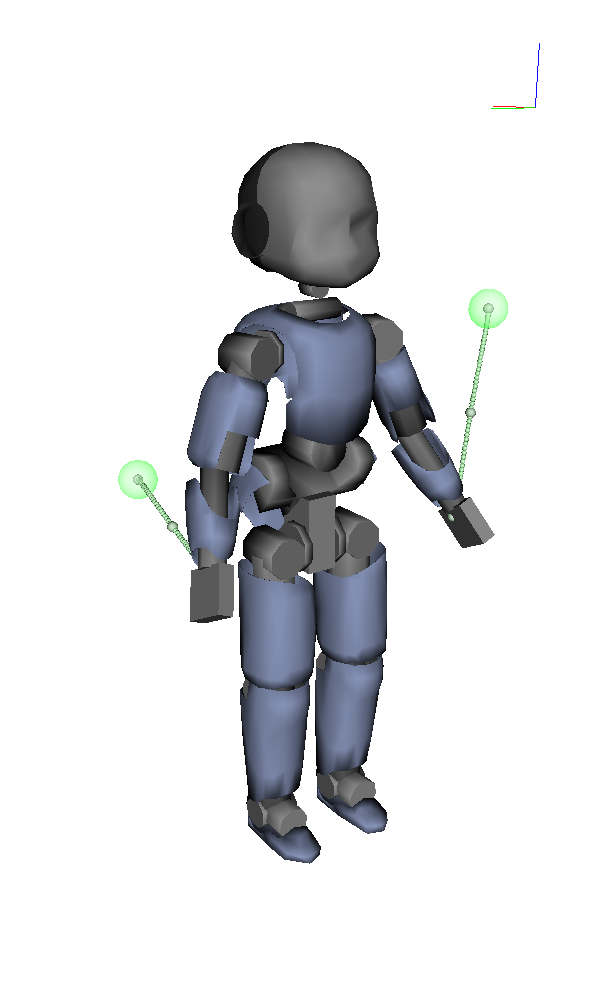
\includegraphics[trim = 0cm 4.5cm 0cm 5cm, clip, height=4 cm]{pics_UPMC/01_starting}
 \caption{Constrained Configuration}
 \label{fig:config}
\end{subfigure}
%

\begin{subfigure}{.31\linewidth}
 \centering
 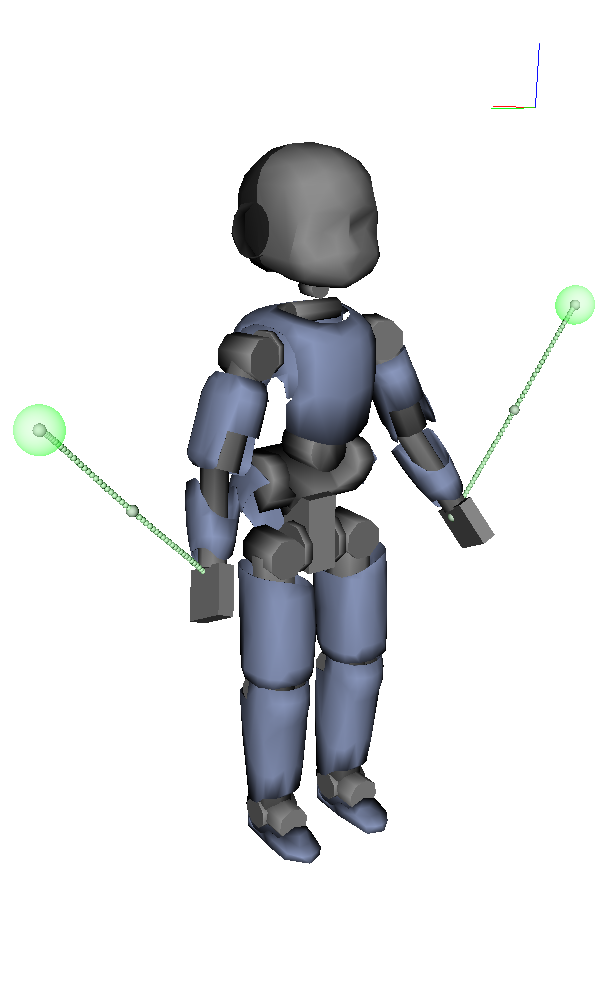
\includegraphics[trim = 0cm 4.5cm 0cm 5cm, clip, height=4 cm]{pics_UPMC/02_starting}
 \caption{Workspace Violation}
 \label{fig:work}
\end{subfigure}
%

\begin{subfigure}{.31\linewidth}
 \centering
 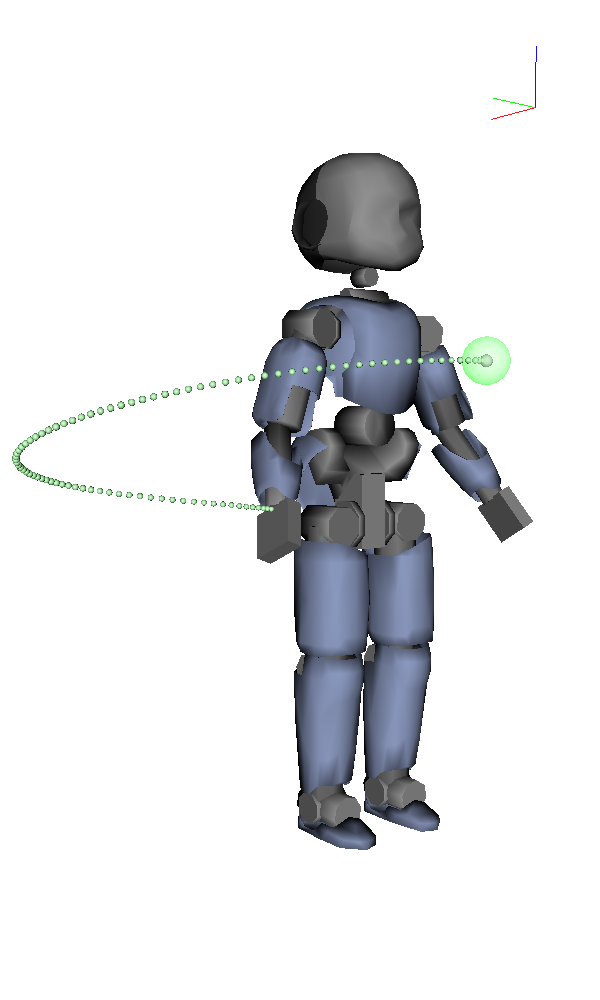
\includegraphics[trim = 0cm 5cm 0cm 5cm, clip, height=4 cm]{pics_UPMC/03_starting}
 \caption{Balance Perturbation}
 \label{fig:balance}
\end{subfigure}
%
\caption{Three common multi-task incompatibility scenarios. The desired hand task trajectories are indicated by the green markers. Medium size spheres represent waypoints, and large transparent spheres represent the final waypoints or goals.}
\label{fig:3_scenarios_lober_2015}
\end{figure*}

% Refs to add to secondYearReport_WP4.bib

%@inproceedings{lober-HUMANOIDS2014,
%    title = {Multiple Task Optimization using Dynamical Movement Primitives for Whole-Body Reactive Control},
%    author = {Lober, R. and Padois, V. and Sigaud, O.},
%    booktitle = {Proceedings of the IEEE-RAS International Conference on Humanoid Robots (Humanoids)},
%    pages = {193-198},
%    doi = {10.1109/HUMANOIDS.2014.7041359},
%    http = {http://hal.archives-ouvertes.fr/hal-01116139/en},
%    year = {2014},
%    month = Nov,
%    address = {Madrid, Spain}
%}

%@inproceedings{lobersubmittedIROS2015,
%    title = {Variance Modulated Task Prioritization in Whole-Body Control},
%    author = {Lober, R. and Padois, V. and Sigaud, O.},
%    booktitle = {Submitted to  the IEEE/RSJ International Conference on Intelligent Robots and Systems},
%    pages = {},
%    doi = {},
%    http = {},
%    year = {2015},
%    month = Sep,
%    address = {Hamburg, Germany}
%}



% 
% %Valerio's paper on learning activation policies in task controller.
% TUD addressed the problem of learning the temporal profile of soft
% task priorities and null-space projectors for the multi-task controllers
% developed in WP3. Our preliminary results have been submitted to a robotics
% conference\footnote{Modugno, V.; Neumann, G.; Rueckert, E.; Oriolo, G.; Peters,
% J.; Ivaldi, S. \textit{Learning soft task prioirities and null-space projectors
% for motion planning of redundant manipulators}. Submitted to IROS 2015.}.
% 
% The first controller of WP3, \textit{Prioritized Task-Space Inverse Dynamics},
% is based on \textit{strict task hierarchies}, where a hierarchical ordering of
% the tasks is set, such that critical tasks (or tasks that are considered as more
% important) are fulfilled with higher priorities, and the low-priority tasks are
% solved in the null-space of the higher priority tasks
% \cite{DelPrete-2014-ID267}. The strict control approach requires the
% pre-specification of the task hierarchy. However, in many contexts it is
% difficult to organize the tasks in a stack and define their relative importance
% in forms of priorities. When priorities are strict, a higher task can completely
% block lower tasks, which can result in movements that are not satisfactory for
% the robot mission (e.g., its ``global'' task). 
% 
% The second controller of WP3 is based on \textit{soft task hierarchies}, where
% the solution is typically given by a combination of weighted tasks
% \cite{Salini-2011-ID348}. The importance or ``soft priority'' of each individual
% task is represented by a scalar weight. By tuning the vector of scalar weights,
% evolving in time, the global robot behavior can be optimized. Within WP3, Liu et
% al. \cite{liu_ICRA2015} propose a generalized projector (GHC) that handles
% strict and non-strict priorities with smooth transitions when tasks priorities
% are swapped. They show that adapting these weights may result in a seamless
% transition between tasks (i.e., reaching for an object, staying close to a
% resting posture and avoiding an obstacle) and in continuous task sequencing.
% Despite the elegant framework, their controller needs again a lot of manual
% tuning: particularly, the evolution of the tasks priorities in time, the timing
% and the tasks transitions need to be designed by hand. While this approach could
% still be easy for few tasks and simple robotic arms, it can quickly become
% unfeasible for complex robots such as humanoids performing whole-body movements
% that usually require a dozen of tasks and constraints (e.g., control balance,
% posture, end-effectors, stabilize head gaze, prevent slipping, control
% interaction forces etc.).
% 
% \begin{figure*}%[t!]
% \centering
% 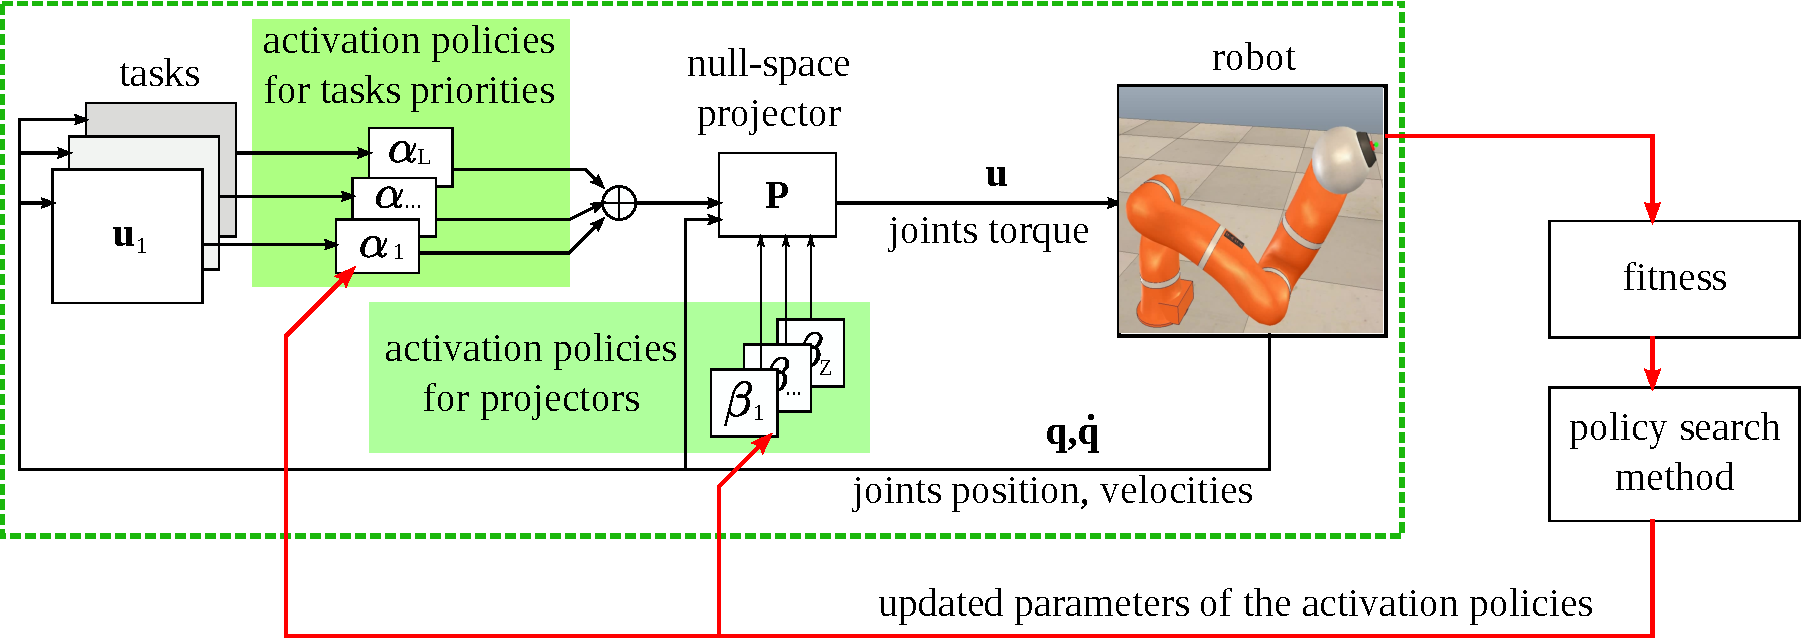
\includegraphics[width=.75\hsize]{./sections/WP4/pics_serena/concept_scheme}
% \caption{This scheme briefly describes the proposed method. The control torques are computed by a combination of tasks weighted by soft priorities, represented as parameterized activation policies, that are multiplied by a Null-space projector, where some activation functions for different projectors are joined. The global task execution is evaluated and a fitness function is computed: a policy search method is then used to optimize the parameters of the activation policies, both for tasks and projector. }
% \label{figure:scheme}
% \end{figure*}
% 
% In this task we propose a first solution to the problem of how these weights can
% be learned through trial-and-error. We study how the \textit{temporal} profiles
% of the task weights can be learned from a reward function, which is assumed to
% be given\footnote{For many robotic task, e.g., tracking desired center-of-mass
% or end-effector trajectories while avoiding obstacles, such reward functions
% have been defined in \cite{Kober_IJRR_2013}.}. 
% 
% As a first step towards a controller that is capable of handling multiple tasks
% and constraints on a complex robot, while allowing us to efficiently learn the
% task priorities, we propose a regularized version of the Unified Framework (RUF)
% proposed by Peters et al \cite{Peters_AR_2008}, where the tasks weights and
% Null space projectors weights are represented by parametrized functional
% approximators that can be automatically determined through a stochastic
% optimization procedure. The concept is presented in Figure~\ref{figure:scheme}.
% 
% \begin{figure}%[b!]
% 
% \begin{subfigure}{.3\textwidth}
%   \centering
%   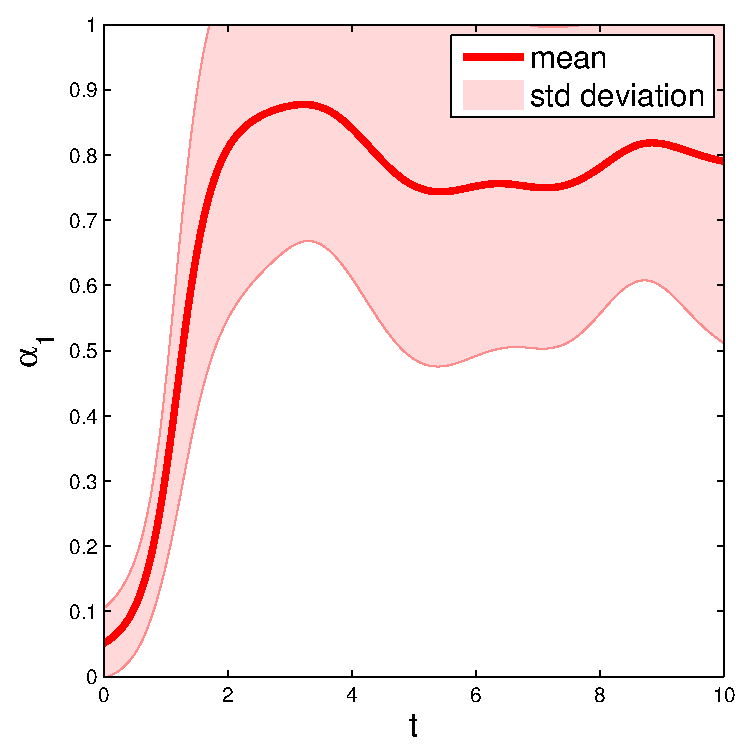
\includegraphics[width=1\linewidth]{./sections/WP4/pics_serena/alpha1}
%   \label{fig:alpha1}
%   \caption{Attractor activation.}
% \end{subfigure}%
% \begin{subfigure}{.3\textwidth}
%   \centering
%   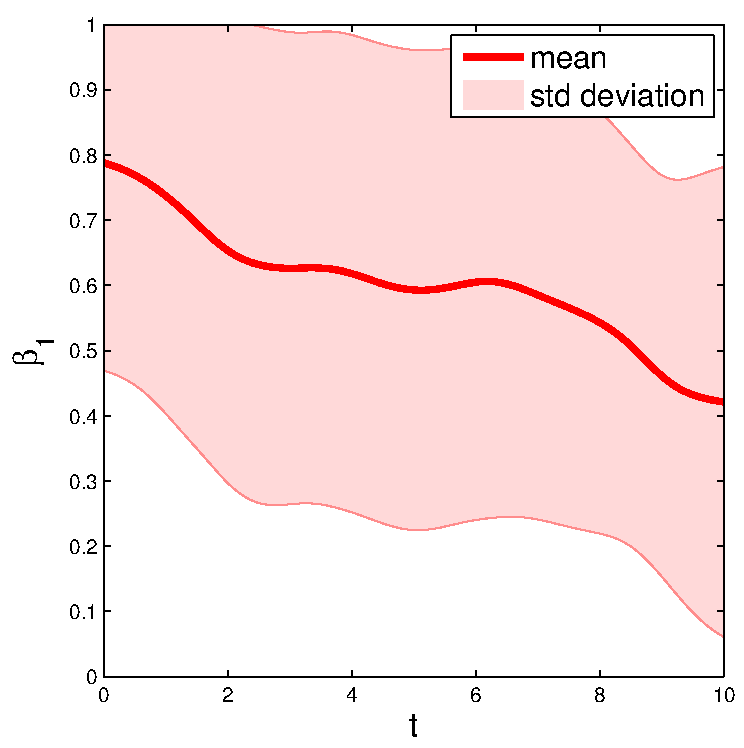
\includegraphics[width=1\linewidth]{./sections/WP4/pics_serena/alpha2}
%   \label{fig:alpha2}
%   \caption{Null-projector activation.}
% \end{subfigure}
% \begin{subfigure}{.38\textwidth}
%   \centering
%   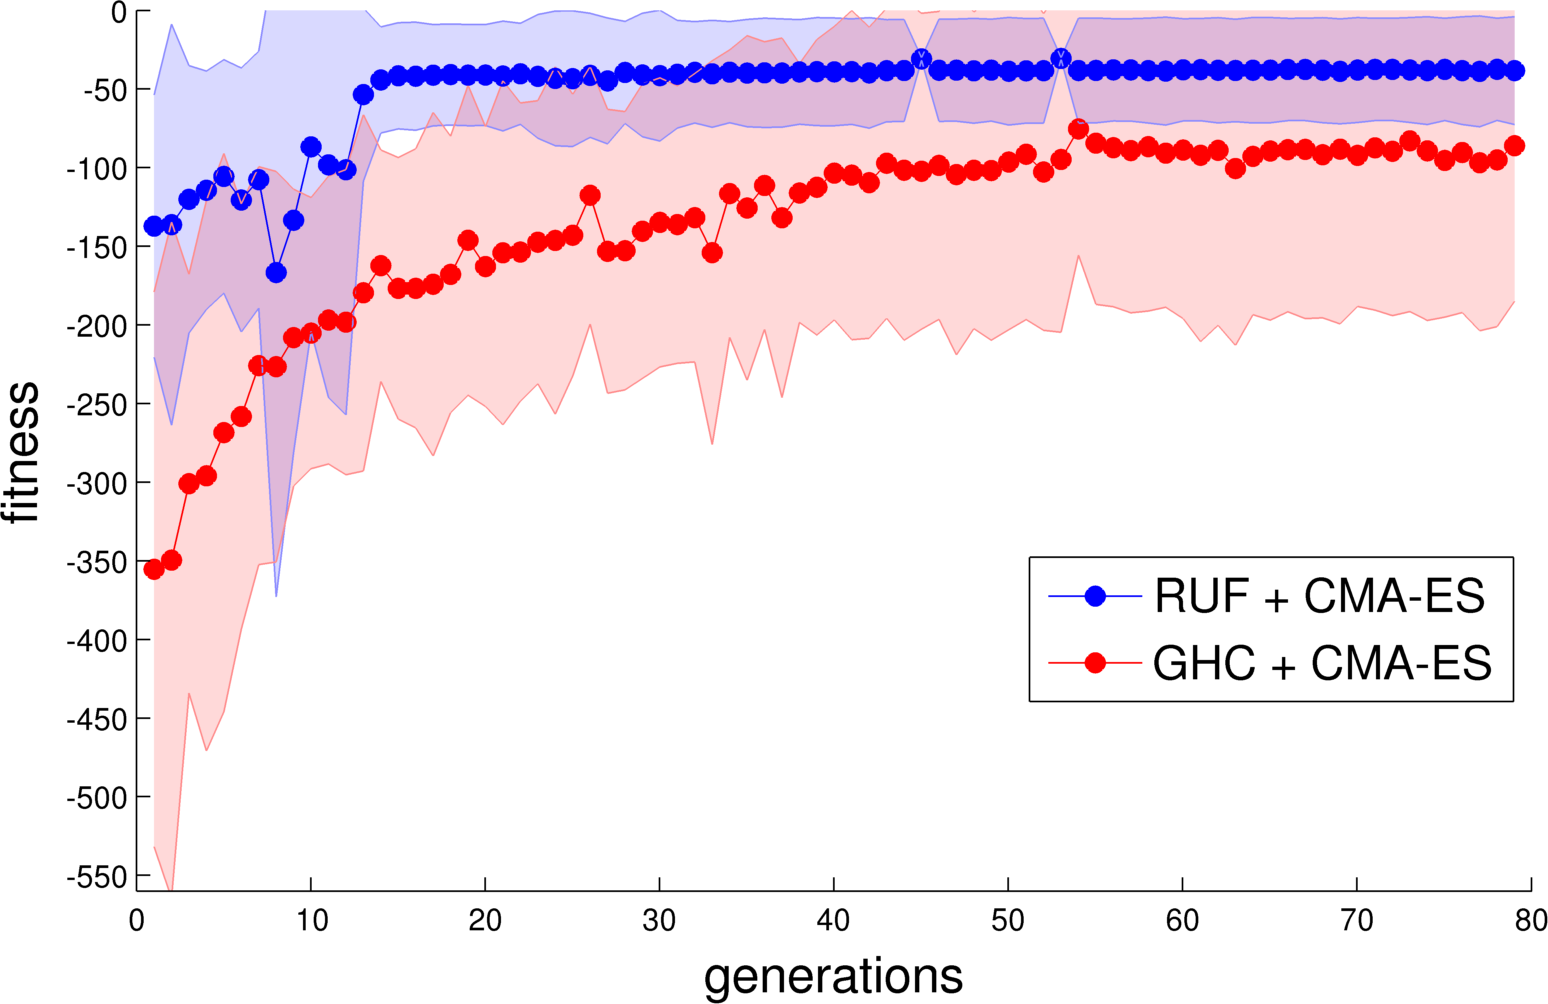
\includegraphics[width=1\linewidth]{./sections/WP4/pics_serena/comparison}
%   \label{fig:alpha3}
%   \caption{Learning performance.}
% \end{subfigure}
% \caption{The panels in (a) and (b) show the mean and standard deviation of the temporal
% profile of the activation functions $\alpha,\beta$, optimized by RUF+CMA-ES,
% computed over $R=50$ replications of the same experiment of the table scenario.
% (c) Comparison of our method (blue line) to the generalized projector method (GHC).}
% \label{fig:activation_policy}
% \end{figure}
% 
% As a first results, we show that the optimization process  generates weights
% profiles that cannot be designed manually in advance, see panels (a) and (b) in 
% Figure~\ref{fig:activation_policy}.
% 
% % \begin{figure}%[b!]
% % \centering
% % 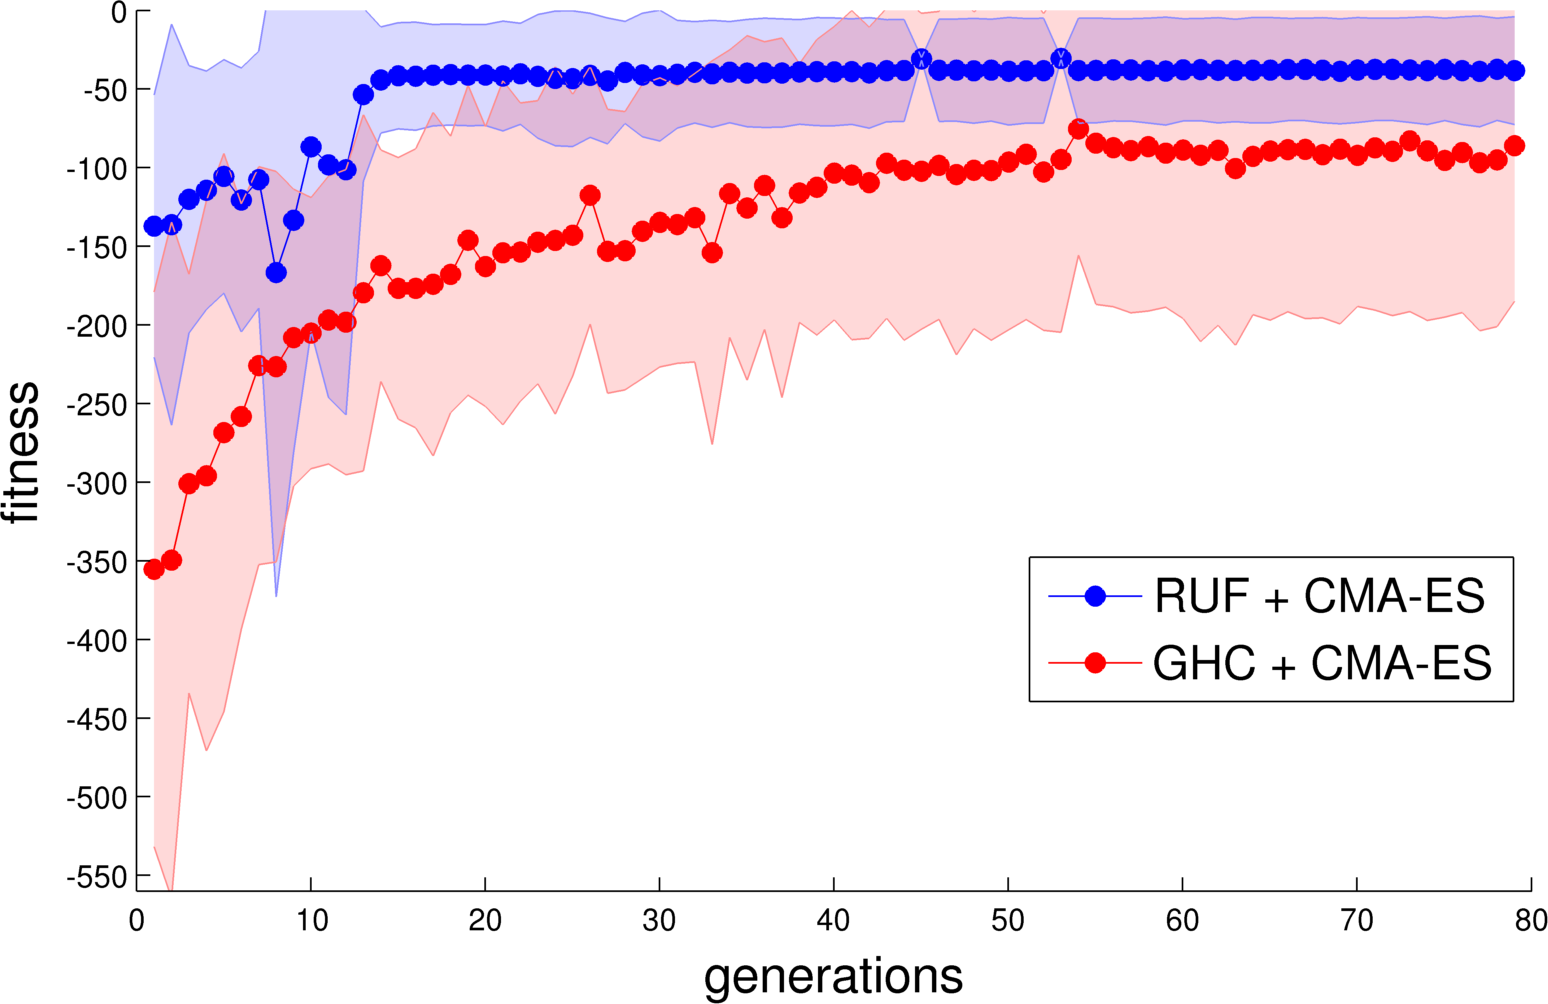
\includegraphics[width=1\hsize]{./sections/WP4/pics_serena/comparison}
% % \caption{This figure shows the mean and the standard deviation of $R=20$
% % replications of the same experiments for our method RUF+CMA-ES and GHC+CMA-ES.
% % For both controllers, we consider a random initial point in the parameter space
% % for the optimization algorithm. Our method shows a faster convergence learning
% % rate and it reaches a better result in terms of the optimized fitness.}
% % \label{fig:comparison}
% % \end{figure}
% 
% We then compare the performance of our controller with the state-of-the-art
% method GHC proposed by Liu et al. \cite{liu_ICRA2015} (WP3). We consider the
% following experimental scenario: a 7-DOF KUKA Light Weight Robot arm, starting
% from a vertical position, must reach a desired point with its end-effector,
% while avoiding to collide with a table, represented by a surface parallel to the
% z-axis in between the robot and the goal. The aim of the experiment is to bring
% the end-effector as close as possible to the desired position, while avoiding
% collisions with the obstacle. We define  $T=3$ tasks: a regulation task in the
% joint space, and two reaching tasks for the elbow and the end-effector. For both
% methods, we find the optimal profiles for the weighting functions with CMA-ES.
% Our second result is that our controller generally performs better than GHC,
% even if we optimize the policies in both methods: on an average of 20
% replicates, our RUF+CMA-ES finds 90\% of the solutions found by our RUF+CMA-ES
% satisfies the constraints, while only 75\% of the solutions of GHC+learning are
% acceptable. Furthermore, the final best solution found by RUF+CMA-ES outperforms
% the one of GHC+CMA-ES, as shown in Figure~\ref{fig:activation_policy} (c).

